\documentclass{gajewski}

\bibliographystyle{IEEEtran}

%%%%%%%%%%%%%%%%%
% Document variables
%%%%%%%%%%%%%%%%%
\docDate{ \today }
\docID{Present cipher}
\docRevision{0.2}
\docStatus{Draft}
\docTitle{\mbox{Present Cipher}} 
\authorName{\mbox{Krzysztof Gajewski} \\ and opencores.org}
\authorURL{www.opencores.org}
\authorAddress{\mbox{}}
\authorEmail{gajos@opencores.org}

\revisionList{ 
0.1 & all & 2014/02/01 & First draft & K. Gajewski \\
0.2 & all & 2014/09/16 & Some small corrections with the text, typos, etc. & K. Gajewski \\
}

\begin{document}

\maketitle

\newpage

\revisionTable

\newpage

\tableofcontents
\newpage

\section{Introduction}

Present is \textgravedbl ultra-lightweight\textacutedbl \space block cipher developed by A. Bogdanov et al. and proposed in 2007 \cite{PRESENT}. It uses 64 bit data block and 80 bit or 128 bit key.
This cipher consists of 32 rounds, during which: 
\begin{itemize}
    \item round key is added to plaintext
    \item plaintext goes through sBoxes (substitution boxes)
    \item plaintext after sBoxes goes through pLayer (permutation layer)
    \item round key is updated
\end{itemize}
After that, ciphertext feeds out the output. Briefly algorithm was shown in Fig. \ref{pAlgorithm}.
\begin{figure}[!ht]%
    \begin{center}
    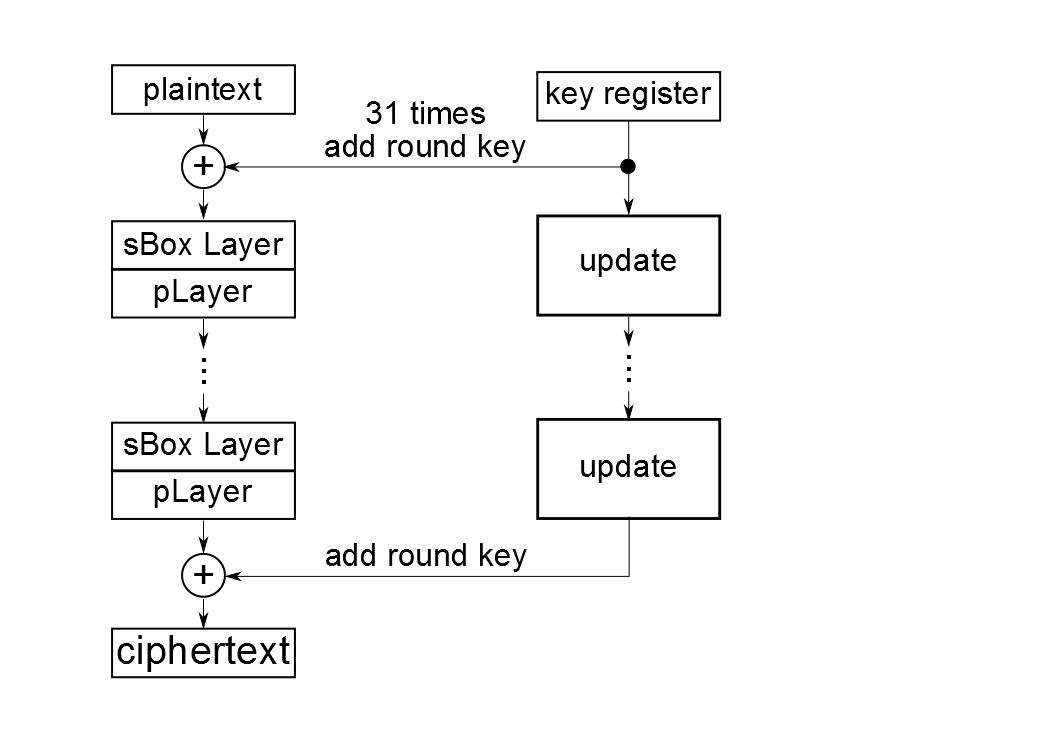
\includegraphics[width=0.66\textwidth]{img/presentAlgorithm.png}
    \caption{%
        Briefly block scheme of the PRESENT block cipher
     }%
    \label{pAlgorithm}
    \end{center}
 \end{figure}
In this project Present block cipher works with 80 bit key. Target was Xilinx\textsuperscript{\textregistered} Spartan 3E XC3S500E \cite{Spartan} on Spartan 3E  Starter Board \cite{Digilent} made by Digilent\textsuperscript{\textregistered}.

\newpage 

\section{Interface}

Top level component of the Present encoder was shown in Fig. \ref{penc}. All inputs and outputs are synchronous except \texttt{reset} signal and sampled at rising edge of the clock. Type for all signals is \texttt{STD\_LOGIC} or \texttt{STD\_LOGIC\_VECTOR}.
\begin{figure}[!ht]%
    \begin{center}
    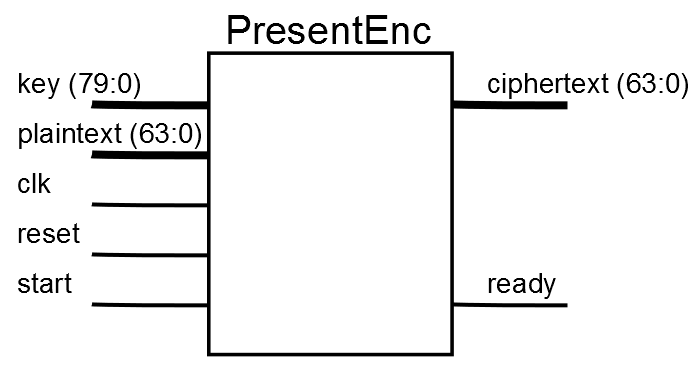
\includegraphics[width=0.5\textwidth]{img/PresentEnc.png}
    \caption{%
        Top level component of the Present encoder
     }%
    \label{penc}
    \end{center}
 \end{figure}

\begin{tabularx}{\textwidth}{|p{30mm}|p{11mm}|p{11mm}|X|}
  \hline \bf{Signal name} & \bf{Width} & \bf{In/Out} & \bf{Description}\\ 
  \hline \texttt{key}	& 80  &  in  & secret key used for input data encoding. \\ 
  \hline \texttt{plaintext}	& 64  &  in  & input data which have to be encoded. \\ 
  \hline \texttt{clk}	& 1  &  in  &  clock signal for the component\\ 
  \hline \texttt{reset} & 1   &  in  & \emph{asynchronous} reset signal.	\\ 
  \hline \texttt{start} & 1   &  in  & signal which starts encoding process. \\ 
  \hline \texttt{ciphertext} & 64   &  out  & encoded text output. \\ 
  \hline \texttt{ready} & 1   &  out  & signal informing about end of encoding process. \newline  "0" - wait until end of data encoding. \newline  "1" - data at the \texttt{ciphertext} output are valid, you can read them. \\ 
  \hline
\end{tabularx}
\captionof{table}{Input/Output signals of the Present encoder }

\newpage

\section{State machine workflow}

Overall internal structure of the Present component is similar to the structure shown in \cite{PRESENT}. Suitable control logic was added in state machine added
to the core. It was shown in Fig. \ref{presentSM}.

\begin{figure}[!ht]%
    \begin{center}
    \includegraphics[width=0.5\textwidth]{img/SM.jpg}
    \caption{%
        State machine of the Present component
     }%
    \label{presentSM}
    \end{center}
 \end{figure}

State machine consist of three states \texttt{NOP}, \texttt{SM\_START} and \texttt{READY}. Some control signal of used multiplexers, registers and counter was omitted. \texttt{NOP} is default state after resetting the core. This state is active as long as \texttt{START} = '0'.

When \texttt{START} = '1' encoding process starts. Proper \texttt{key} and \texttt{plaintext} must feed the input before start encoding. \texttt{SM\_START} state is active as long as \texttt{START} = '1'. Change of this signal to '0' automatically stops encoding process. 

After 32 clock cycles (counter reach \texttt{'11111'} value), when the encoding process is ends, state machine automatically change its state to \texttt{READY}. This informs user by setting \texttt{READY} output to '1'. Then \texttt{ciphertext} output contains proper data, which can be read by user. This state is active as long as \texttt{START} = '1'. Change this signal to '0', turns the state machine to \texttt{NOP} state. Core is ready for the next data encoding.

\newpage

\section{FPGA implementations}

The  component  has  only  been  verified on a Xilinx\textsuperscript{\textregistered} Spartan 3E XC3S500E FPGA in FG320 package and synthesized  with  Xilinx  ISE  14.2.  Appropriate setup files was prepared with the use of ISE Project Navigator, but Makefile scripts was also written. Suitable files was stored in \texttt{./Pure/syn/XC3ES500/}  directory. 
Implementation in FPGA device was done in another subproject called \texttt{PureTesting}.
Makefile was tested in Windows 8 with use of Cygwin for 64-bit Windows.

Synthesis results was given in Fig. \ref{SynResults}

\begin{tabularx}{\textwidth}{|p{45mm}|p{30mm}|p{30mm}|X|}
  \hline \multicolumn{4}{|c|}{Xilinx \textregistered Spartan 3E XC3S500E FPGA in FG320 package} \\
  \hline \bf{Parameter} & \bf{Used} & \bf{Available} & \bf{Utilization}\\ 
  \hline Number of Slices & 248 & 4656 & 5\% \\
  \hline Number of Slice Flip Flops & 151 & 9312 & 1\% \\
  \hline Number of 4 input LUTs & 296 & 9312 & 3\% \\
  \hline Number of bonded IOBs & 212 & 232 & 91\% \\
  \hline Number of GCLKs & 1 & 24 & 4\%\\
  \hline Minimum period & 5.035ns & - & - \\
  \hline Maximum Frequency & 198 MHz & - & - \\
  \hline
\end{tabularx}
\label{SynResults}
\captionof{table}{Synthesis results for Spartan 3E XC3S500E}

Possible change in used FPGA device may be possible in steps given below\footnotemark[1]:
\begin{enumerate}
    \item Copy \texttt{./Pure/syn/XC3ES500/} directory to another one like \texttt{./Pure/syn/YOUR\_FPGA\_SYMBOL/}
    \item Go to \texttt{./Pure/syn/YOUR\_FPGA\_SYMBOL/}  directory.
    \item In \texttt{PresentEnc.xst} file modify the line \texttt{-p xc3s500e-5-fg320} to \texttt{-p YOUR\_FPGA\_CODE}
    \item In \texttt{Makefile} file modify the line \texttt{PLATFORM=xc3s500e-fg320-5} to \texttt{PLATFORM=YOUR\_FPGA\_CODE}
\end{enumerate}

\footnotetext[1]{This solution was not tested and is based on my own observations.}


\newpage

\section{Simulation}

Self-checking test bench were provided to the components used for Present encoder. They are stored in \texttt{./Pure/bench/vhdl} directory. Suitable configuration files and Makefile used for running test bench was stored in 
\texttt{.Pure/sim/rtl\_sim/bin} directory. Appropriate test vectors was taken from \cite{PRESENT}.

Makefile was prepared to make "manual run" of tests. If You want to perform it without gui, remove \texttt{-gui} option in Makefaile.

\newpage

\section{Troubleshooting}

During work with Windows 8 64-bit and and Xilinx\textsuperscript{\textregistered} ISE 64-bit some problems may occur:

\begin{enumerate}
    \item Xilinx may be unable to open projects in Project Navigator.
    \item When you run \texttt{make} in Cygwin and perform testbench it would be unable to open ISIM gui.
    \item When you run ISIM gui  (*.exe test bench file) it hangs out or anti virus protection opens.
\end{enumerate}

To solve problems listed above you have to perform steps listed below:
\begin{enumerate}
    \item You have to rename libraries \texttt{libPortabilityNOSH.dll} to \texttt{libPortability.dll} from \texttt{nt64} directories (\href{http://www.gadgetfactory.net/2013/09/having-problems-installing-xilinx-ise-on-windows-8-64bit-here-is-a-fix-video-included/}{http://www.gadgetfactory.net/2013/09/having-problems-installing-xilinx-ise-on-windows-8-64bit-here-is-a-fix-video-included/})
    \item Firstly, install Cygwin X11 (\href{http://stackoverflow.com/questions/9393462/cannot-launch-git-gui-using-cygwin-on-windows}{http://stackoverflow.com/questions/9393462/cannot-launch-git-gui-using-cygwin-on-windows})
    \item Temporary switch off anti virus protection.
\end{enumerate}

\newpage

\section{License and Liability}

Copyright \textcopyright  2013 Authors and OPENCORES.ORG

This source file may be used and distributed without
restriction provided that this copyright statement is not
removed from the file and that any derivative work contains
the original copyright notice and the associated disclaimer.

This source file is free software; you can redistribute it
and-or modify it under the terms of the GNU Lesser General
Public License as published by the Free Software Foundation;
either version 2.1 of the License, or (at your option) any
later version.

This source is distributed in the hope that it will be
useful, but WITHOUT ANY WARRANTY; without even the implied
warranty of MERCHANTABILITY or FITNESS FOR A PARTICULAR
PURPOSE. See the GNU Lesser General Public License for more
details.

You should have received a copy of the GNU Lesser General
Public License along with this source; if not, download it
from \href{http://www.opencores.org/lgpl.shtml}{http://www.opencores.org/lgpl.shtml}

Xilinx, Spartan3E is registered trademark of Xilinx Inc. 2100 Logic Drive, San Jose CA USA

\newpage

\bibliography{bibliography}

\end{document}
